\documentclass[a5paper]{article}

\usepackage{amsmath, amssymb}
\usepackage{multicol}
\setlength{\columnsep}{1cm}
\usepackage[margin=0.75in]{geometry}
\usepackage{graphicx}
\graphicspath{ {../../../Images/COIT11240/} }
\usepackage[breaklinks, hidelinks]{hyperref}
\usepackage{siunitx}
\usepackage{tikz}
\usetikzlibrary{patterns, positioning, arrows.meta, matrix, fit}
\usepackage{xcolor}
\usepackage[american]{circuitikz}
\usepackage{pgfplots}
\pgfplotsset{compat=newest}
\usepgfplotslibrary{external}
\usepackage{stix}
\usepackage{ragged2e}
\usepackage{enumitem}
\usepackage{polynom}

\newcommand{\minus}{\scalebox{0.5}[1.0]{$-$}}
\newcommand{\sech}{\mathrm{sech}}
\newcommand{\csch}{\mathrm{csch}}
\newcommand{\Lap}{\mathcal{L}}
\setcounter{secnumdepth}{4}
\renewcommand\paragraph{\@startsection{paragraph}{4}{\z@}%
% display heading, like subsubsection
                                     {-3.25ex\@plus -1ex \@minus -.2ex}%
                                     {1.5ex \@plus .2ex}%
                                     {\normalfont\normalsize\bfseries}}
\sisetup{
	round-mode = places,
	round-precision = 2,
}

\date{24\textsuperscript{th} of September 2026}

\begin{document}
	\begin{titlepage}
		\centering
		{\Huge \textsc{COIT11240 - Dashboard Design}\par}
		\vspace{1cm}
		{\Large \textsc{Lecture Notes}\par}
		\vspace{2.5cm}
		\vfill
		Authored by\par
		Lachlan J. W. Wyer
		\vfill
		\makeatletter
		{\large Document Start Date: \@date \par}
		\makeatother
		{\large Latest Update: \today\par}
	\end{titlepage}
	\tableofcontents
	\pagebreak

	\section{Signals and Times Systems}
	\subsection{Signals:}
	A signal is a physical quantity that varies by something. The most common ones are time, space, and angle. Basically if it ca be measured or its effects measured, it can be though of as a signal. For example:
	\begin{itemize}
		\item Radio waves
		\item AC waveform
		\item Temperature
		\item Tide height
		\item Digital bit streams
	\end{itemize}
	\subsection{Continuous vs. Discrete:}
	A continuous signal has a value for all time points. A waveform with considered infinite precision.
	\begin{center}
	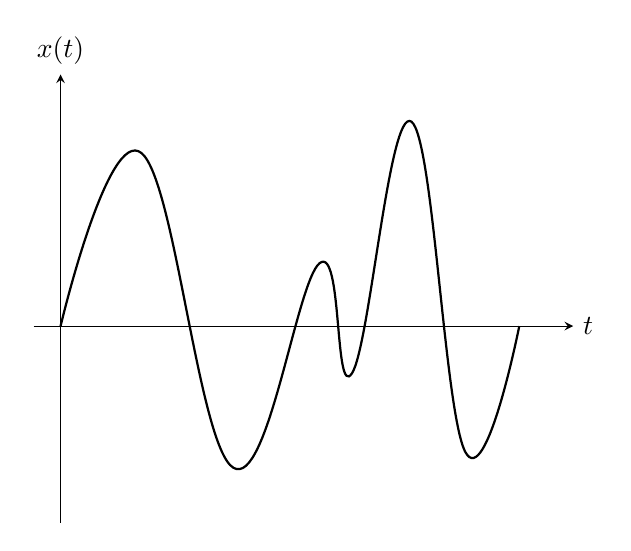
\begin{tikzpicture}
	\begin{axis}[
	    axis lines=middle,
	    xlabel={$t$},
	    ylabel={$x(t)$},
	    xmin=-0.5, xmax=9.5,
	    ymin=-2.5, ymax=3.2,
	    ticks=none,
	    every axis x label/.style={at={(current axis.right of origin)}, anchor=west},
	    every axis y label/.style={at={(current axis.above origin)}, anchor=south}
	]
	    % Continuous smooth waveform
	    \addplot+[thick, black, mark=none, smooth, tension=0.7] coordinates {
		(0, 0)
		(1.5, 2.2)
		(3.2, -1.8)
		(4.8, 0.8)
		(5.4, -0.6)
		(6.5, 2.6)
		(7.5, -1.6)
		(8.5, 0)
	    };
	\end{axis}
	\end{tikzpicture}
	\end{center}
	Discrete signalling on the other hand, only has values at set time points.
	\begin{center}
	\begin{tikzpicture}
	\begin{axis}[
	    axis lines=middle,
	    xlabel={$n$},
	    ylabel={$x[n]$},
	    xmin=-0.5, xmax=7.8,
	    ymin=-2.5, ymax=3.5,
	    xtick={1,2,3,4,5,6,7},
	    ytick=\empty,
	    every axis x label/.style={at={(current axis.right of origin)}, anchor=west},
	    every axis y label/.style={at={(current axis.above origin)}, anchor=south}
	]
	    % Stem plot using unfilled circular markers (mark=o)
	    \addplot+[ycomb, mark=o, thick, black] coordinates {
		(1, 2.5)
		(2, 1.5)
		(3, 0.0)
		(4, -2.0)
		(5, -1.0)
		(6, 1.5)
		(7, -1.2)
	    };
	\end{axis}
	\end{tikzpicture}
	\end{center}
	\subsection{Sampling:}
	A discrete signal can be made by sampling a continuous signal of set time intervals. The sampled frequency must be twice the continuous frequency, as a minimum. The high the sampled frequency, the more accurate the output waveform.
	\subsection{Nyquist Theorem:}
	If a function $x(t)$ contains a highest frequency of BHz. For it too be completely determined sampling must be done at $\frac{1}{2B}$s.
	\subsection{System:}
	A group of regular items interacting to form a while. Such as, power amp, transformer, or laptop.
	\subsection{Signal Transformation:}
	\subsubsection{Amplitued Transform}
	Scaling the signal
	$$x(t)\rightarrow ax(t)$$
	\subsubsection{Amplitude Shift}
	Vertical shift
	$$x(t)\rightarrow x(t)+b$$
	\subsubsection{Time Reversal}
	A flip across the $y$-axis
	$$x(t)\rightarrow x(-t)$$
	\subsubsection{Time Scaling}
	Changing the frequency
	$$x(t)\rightarrow x(bt)$$
	\begin{itemize}
		\item If $b>1$: Compressing the signal
		\item Else $0<b<1$: Expanded the signal
	\end{itemize}
	\subsubsection{Time Shifting}
	Horizontal movement
	$$x(t)\rightarrow x(t-t_{0})$$
	\begin{itemize}
		\item If $t_{0}>0$: Shifts signal right
		\item Else $t_{0}<0$: Shifts signal left
	\end{itemize}
	\subsection{Even and Odd Signals:}
	Even signals are symmetric around the origin.
	$$x(t)=x(-t)$$
	Odd signals are asymmetric.
	$$x(t)=-x(-t)$$
	Any signal can be decomponsed into even and odd components.
	$$x_{e}(t)=\frac{1}{2}[x(t)+x(-t)]$$
	$$x_{o}(t)=\frac{1}{2}[x(t)-x(-t)]$$
	Sub $t=-t$, into even components.
	\begin{align*}
		x_{e}(-t)&=\frac{1}{2}[x(-t)+x(-(-t))]\\
		&=\frac{1}{2}[x(t)+x(-t)]\\
		&=x_{e}(t)\\
		&\therefore\text{Even}
	\end{align*}
	Sub $t=-t$, into odd components.
	\begin{align*}
		x_{o}(-t)&=\frac{1}{2}[x(-t)-x(-(-t))]\\
		&=\frac{1}{2}[-x(t)+x(-t)]\\
		&=-\frac{1}{2}[x(t)-x(-t)]\\
		&=-x_{o}(t)\\
		&\therefore\text{Odd}
	\end{align*}
	$$x(t)=x_{e}(t)+x_{o}(t)$$
	\subsection{Periodic Signals:}
	$$x(t)=x(t+T_{0}),\;T_{0}>0$$
	This is where $T_{0}$ is the period.
	\subsubsection{Complex Form}
	\begin{align*}
		x(t)&=e^{j\omega_{0}(t+T_{0})}\\
		&=e^{j\omega_{0}t}e^{j\omega_{0}T_{0}}
	\end{align*}
	\subsubsection{Fundamental Period}
	$$T_{0}=\frac{2\pi}{\omega_{0}}$$
	\subsection{General Complex Exponential:}
	$$C=|C|e^{j\phi},\;\;\;a=r+j\omega$$
	\begin{align*}
		x(t)&=|C|e^{j\phi(r+j\omega_{0})t}\\
		&=|C|e^{rt}e^{j\phi}e^{j\omega_{0}t}
		&=|C|e^{rt}\cos{(\omega_{0}t+\phi)}+j|C|e^{rt}\sin{(\omega_{0}t+\phi)}
	\end{align*}
	\subsection{Step Function:}
	Switching operations require abrupt changes in $v(t)$ and $t$. At the switching point, it is undefined.
	\begin{align*}
		Ku(t)=0,\;t<0\\
		Ku(t)=K,\;t>0\\
		Ku(t)=undf,\;t=0
	\end{align*}
	\subsection{Impulse Function:}
	This function has infinite magnitude and zero duration. No practical application contains this, as nothing last with zero time. It is used to define derivative at discontinuity point. Discrete signals can be saved to be made up of multiple impulse functions.
	$$x[n]=\sum^{k=\inf}_{k=-\inf}x[k]\delta[n-k]$$
	\subsection{Signal Energy and Power:}
	\subsubsection{Continuous}
	$$E=\int^{t_{2}}_{t_{1}}|x(t)|^{2}dt$$
	$$P=\frac{1}{t_{2}-t_{1}}\int^{t_{2}}_{t_{1}}|x(t)|^{2}dt$$
	$$E_{\infty}=\lim_{T\to\infty}\int^{T}_{-T}|x(t)|^{2}dt$$
	$$P_{\infty}=\lim_{T\to\infty}\frac{1}{2T}\int^{T}_{-T}|x(t)|^{2}dt$$
	\subsubsection{Discrete}
	$$E=\sum^{n_{2}}_{n_{1}}|x[n]|^{2}$$
	$$P=\frac{1}{n_{2}-n_{1}}\sum^{n_{2}}_{n_{1}}|x[n]|^{2}$$
	$$E_{\infty}=\lim_{N\to\infty}\sum^{N}_{-N}|x[n]|^{2}$$
	$$P_{\infty}=\lim_{N\to\infty}\frac{1}{2N+1}\sum^{N}_{-N}|x[n]|^{2}$$
	\subsubsection{Fundamentals}
	If energy over an infinite interval is finite, $E_{\infty}<\infty$, then $P_{av}$ is 0, $P_{\infty}=0$. Else $P_{\infty}>0\;\;\rightarrow\;\;E_{\infty}=\infty$. A few cases can have $E_{\infty}=\infty$ and $P_{\infty}=\infty$. One such one is $x(t)=t$.
	\subsection{System Representation:}
	A system is usually represented by a black box.
	\begin{center}
	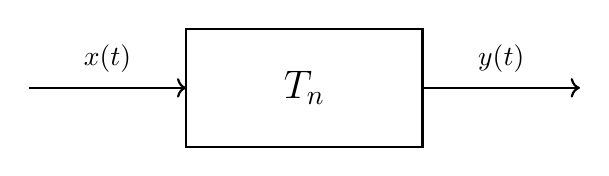
\begin{tikzpicture}
	    % System Block
	    \draw[thick] (2, -0.75) rectangle (5, 0.75);
	    \node at (3.5, 0) {\Large $T_n$};

	    % Input Arrow & Label
	    \draw[->, thick] (0, 0) -- (2, 0) node[midway, above=2pt] {$x(t)$};

	    % Output Arrow & Label
	    \draw[->, thick] (5, 0) -- (7, 0) node[midway, above=2pt] {$y(t)$};
	\end{tikzpicture}
	\end{center}
	$$y(t)=T_{n}[x(t)]$$
	The $T_{n}$ is not a function but a transformation happening to the function.
	\subsection{Causality:}
	A system is casual if it only depends on present and past values.
	$$y(t)=5x(t)=6x^{2}(t-1)+y(t-1)$$
	\subsection{Invertability:}
	A system is said to be invertible if the operations placed on it can be revered, giving a unique answer.
	\subsubsection{Invertable}
	\begin{align*}
		y[n]&=2x[n]\\
		x[n]&=\frac{1}{2}y[n]\\\\
		y(t)&=\int^{t}_{-\infty}x(\tau)d\tau\\
		x(t)&=\frac{dy(t)}{dt}
	\end{align*}
	\subsubsection{Non-Invertable}
	\begin{align*}
		y(t)&=x^{2}(t)\\
		x(t)&=\pm\sqrt{y(t)}\\
		&\text{Produces 2 possible results}\\\\
		y[n]=nx[n]\\
		x[n]=\frac{1}{n}y[n]\\
		\text{Non result if }&n\neq0
	\end{align*}

	\section{Linear Time Invariant Systems}
	\subsection{What are They?:}
	A linear system is one which obeys the laws of linearity and superposition:
	\begin{itemize}
		\item If $x$ is multiplied by $k$ making $kx$, $f(x)$ is also now $kf(x)$.
		\item When more than one factor is applied it is the sum of individual responses to each input.
	\end{itemize}
	\subsection{Time Invarience:}
	Behaviour and characteristic of the system is fixed over time. An example of this is an RC circuit characteristics will not change if the experiment is conducted today, tomorrow or yesterday. Mathematically, if the input is shifted by $T$, the output is also shifted by $T$.
	$$x(t)\Rightarrow y(t)$$
	$$x(t-T)\Rightarrow y(t-T)$$
	\subsection{Discrete Signals as Impulse Functions:}
	$$x[n]=\sum^{\infty}_{k=-\infty}x[k]\delta[n-k]$$
	For any given value of $n$, only 1 impulse in non-zero, and the rest are zero. Assume the response of an LTI system to unit impulse  $\delta[n]$ is $h[n]$. Thus $\delta[n-k]$ is $h[n-k]$.
	\subsection{Convolution of Discrete Signals:}
	The response of that system to signal $n[n]$ is superposition of a scaled and time shifted $h[n]$.
	$$y[n]=\sum^{\infty}_{k=-\infty}x[k]h[n-k]$$
	This is often called the convoluetion sum.
	\begin{align*}
		y[n]=&x[n]\otimes h[n]\\
		=&\sum^{\infty}_{k=-\infty}x[k]h[n-k]
	\end{align*}
	\begin{center}
	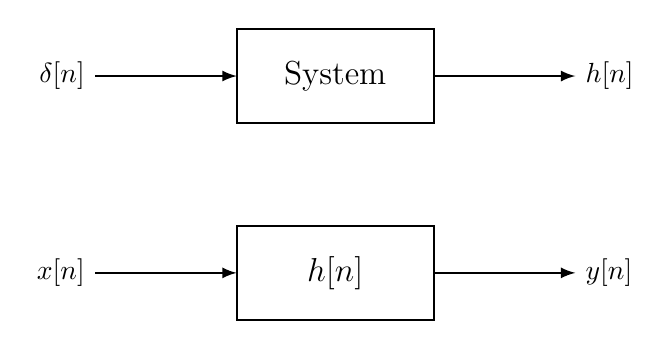
\begin{tikzpicture}[>=latex]
	    % --- Top Block: Impulse Response Definition ---
	    \draw[thick] (2, 1.4) rectangle (4.5, 2.6);
	    \node at (3.25, 2) {\large System};
	    \draw[->, thick] (0.2, 2) node[left] {$\delta[n]$} -- (2, 2);
	    \draw[->, thick] (4.5, 2) -- (6.3, 2) node[right] {$h[n]$};

	    % --- Bottom Block: LTI System Characterization ---
	    \draw[thick] (2, -1.1) rectangle (4.5, 0.1);
	    \node at (3.25, -0.5) {\large $h[n]$};
	    \draw[->, thick] (0.2, -0.5) node[left] {$x[n]$} -- (2, -0.5);
	    \draw[->, thick] (4.5, -0.5) -- (6.3, -0.5) node[right] {$y[n]$};
	\end{tikzpicture}
	\end{center}
	\subsection{Convolution Sum-Table Method:}
	Let:
	$$x[n]={2,1,-1,-2,-3}$$
	$$h[n]={1,2,0,-3}$$
	$$x[0]=-1,\;\text{and}\;h[0]=2$$
	\begin{center}
	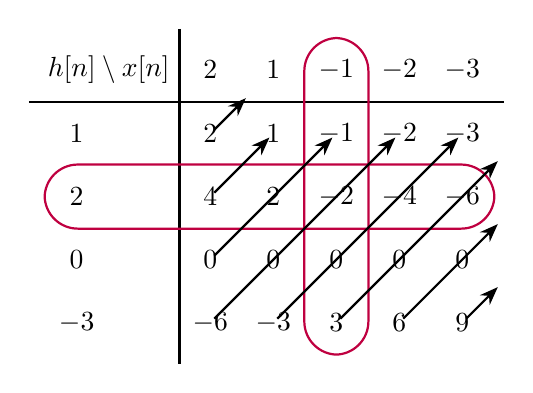
\begin{tikzpicture}[>=Stealth]
	    % Convolution Matrix Table
	    \matrix (m) [
		matrix of math nodes,
		nodes={minimum size=8mm, anchor=center},
		column 1/.style={nodes={anchor=east}},
		row 1/.style={nodes={anchor=south}}
	    ] {
		h[n] \setminus x[n] &  2 &  1 & -1 & -2 & -3 \\
		1                   &  2 &  1 & -1 & -2 & -3 \\
		2                   &  4 &  2 & -2 & -4 & -6 \\
		0                   &  0 &  0 &  0 &  0 &  0 \\
	       -3                   & -6 & -3 &  3 &  6 &  9 \\
	    };

	    % Straight Horizontal and Vertical Table Boundary Lines
	    \draw[thick] (m.west |- m-1-1.south) -- (m.east |- m-1-1.south);
	    \draw[thick] (m-1-1.east |- m.north) -- (m-1-1.east |- m.south);

	    % Purple Unfilled Highlight Loops
	    \node[draw=purple, thick, rounded corners=12pt, fit=(m-3-1)(m-3-6), inner sep=0pt] {};
	    \node[draw=purple, thick, rounded corners=12pt, fit=(m-1-4)(m-5-4), inner sep=0pt] {};

	    % Anti-diagonal Summation Arrows (Bottom-Left to Top-Right)
	    \begin{scope}[->, thick, shorten >=2pt, shorten <=2pt]
		\draw (m-2-2.center) -- ++(0.5,0.5);
		\draw (m-3-2.center) -- (m-2-3.center);
		\draw (m-4-2.center) -- (m-2-4.center);
		\draw (m-5-2.center) -- (m-2-5.center);
		\draw (m-5-3.center) -- (m-2-6.center);
		\draw (m-5-4.center) -- (m-3-6.center) -- ++(0.5,0.5);
		\draw (m-5-5.center) -- (m-4-6.center) -- ++(0.5,0.5);
		\draw (m-5-6.center) -- ++(0.5,0.5);
	    \end{scope}
	\end{tikzpicture}
	\end{center}
	$$y[n]={2,4,1,-10,-10,-3,6,9}$$
	$$y[0]=-10$$
	\begin{center}
	\begin{tikzpicture}[>=latex]
	    % Axes with arrows at both ends
	    \draw[<->, thick] (-4.2, 0) -- (5.2, 0) node[right] {$n$};
	    \draw[<->, thick] (0, -3.8) -- (0, 3.8) node[above] {$y[n]$};

	    % Discrete impulses with arrowheads
	    % Value mapping: (x-coordinate / display-value / visual-y-height)
	    \foreach \pos/\val/\h in {-3/2/0.8, -2/5/1.8, -1/1/0.4, 0/-10/-3.0, 1/-10/-3.0, 2/-3/-1.1, 3/6/2.2, 4/9/3.1} {
		% Stem arrow
		\draw[->, thick] (\pos, 0) -- (\pos, \h);
		
		% Value labels
		\ifdim \h cm > 0cm
		    \node[above=1pt] at (\pos, \h) {\small $\val$};
		\else
		    \node[below=1pt] at (\pos, \h) {\small $\val$};
		\fi

		% X-axis tick labels
		\ifnum \pos=0
		\else
		    \node[anchor=south east, font=\small] at (\pos, 0) {$\pos$};
		\fi
	    }
	    
	    % Origin label
	    \node[below left=2pt, font=\small] at (0, 0) {$0$};
	\end{tikzpicture}
	\end{center}
	\subsection{Convolution Sums Graphical Representation:}
	\begin{itemize}
		\item Draw input signal as a function of $k$
		\item Draw impulse responses as function of $k$
		\item Time reverse the impulse response
		\item Shift impulse along $t$-axis
		\item For each $n$ take the sum of product between input and shifted overlaps
	\end{itemize}
	\subsection{Continuous Time Signals:}
	Any continuous time signal can be approximated by a thin set of strips, known as staircase approximations. The height of the strip, $\hat{x}(t)$, is the value of $x(t)$ at the start of the strip.
	\subsection{Pulse Function:}
	\begin{equation*}
		p(t)=
		\left\{\begin{array}{lr}
			\frac{1}{\Delta t},\;0<t<\Delta t\\
			0,\;\text{Elsewhere}
		\end{array}\right\}
	\end{equation*}
	\begin{center}
	\begin{tikzpicture}[>=latex]
	    % Axes
	    \draw[->, thick] (-0.5, 0) -- (4, 0) node[right] {$t$};
	    \draw[->, thick] (0, -0.5) -- (0, 3);

	    % Rectangular Pulse (Unfilled)
	    \draw[thick] (0, 2) -- (2.5, 2) -- (2.5, 0);

	    % Axis Ticks & Labels
	    \node[below left] at (0, 0) {$0$};
	    \node[below] at (2.5, 0) {$\Delta t$};
	    \node[left] at (0, 2) {$\frac{1}{\Delta t}$};
	\end{tikzpicture}
	\end{center}
	$$\int^{\infty}_{-\infty}p(t)dt=t$$
	\subsection{Continuous Time Series Approximation:}
	This can be approximated as a series of pulse functions.
	\begin{itemize}
		\item Pulse located at integral multiples of pulse width ($\Delta t$)
		\item Pulse height is $x(\Delta t)$
	\end{itemize}
	Pulse of $t=\Delta t$.
	$$x(k\Delta t)[p(t-k\Delta t)\cdot\Delta t]=x(\Delta t)$$
	The signal can then be approximated as the sum of these signals.
	$$\hat{x}(t)=\sum^{\infty}_{k=-\infty}x(k\Delta t)[p(t-k\Delta t)\cdot\Delta t]$$
	As $\Delta t\to0$, $p(t)$ approaches an impulse function.
	$$x(t)=\int^{\infty}_{\infty}x(\tau)\delta(t-\tau)d\tau$$
	As $\Delta t\to0$, $k\Delta t\to\tau$, $\Delta t\to d\tau$ and $p(t-k\Delta t)\to\delta(t-\tau)$.
	\subsection{Pulse Response:}
	If $h(t)$ is the response to the LTI system, $h_{p}(t)$ can be defined to be the response of a pulse system.

	\section{Laplace Transformation}
	\subsection{Why Laplace?:}
	\begin{itemize}
		\item Solving linear circuits frequently involves solving linear differential \\equations. These include transient analysis, AC analysis and transient or steady state system response.
		\item Finding time domain convolution
		\item Signals with many freqency components may be more apparent in a different domain
	\end{itemize}
	\subsection{Laplace Transform:}
	$$\Lap\{f(t)\}=F(s)=\int^{\infty}_{0}f(t)e^{-st}dt$$
	\begin{itemize}
		\item Convert a time domain function to frequency domain. $t\Rightarrow s,\;\text{where}\;s=\sigma+j\omega$
		\item Important Notes
		\begin{itemize}
			\item If intergrand does not converge there is no Laplace transform
			\item Only currently $t>0^{-}$
		\end{itemize}
	\end{itemize}
	\subsection{Conventions:}
	\begin{center}
	\begin{tabular}{ c c c }
		Time domain & & Frequency Domain\\
		$f(t)$ & $\Rightarrow$ & $F(s)$\\
		$g(t)$ & $\Rightarrow$ & $G(s)$
	\end{tabular}
	\end{center}
	Functional transform is only specific functions. Operation transofmr is the description of how mathematical operations are done using Laplace.
	\subsection{Integration by Parts:}
	$$\int^{\infty}_{0}uv'dt=[uv]^{\infty}_{0}-\int^{\infty}_{0}u'vdt$$
	Make sure that $u$ simplifies when derived and $v'$ simplifies when integrated. Laplace transform of 1:
	\begin{align*}
		\Lap\{f(t)\}&=F(s)=\int^{\infty}_{0}f(t)e^{-st}dt\\
		\Lap\{1\}&=\int^{\infty}_{0}e^{-st}dt\\
		&=[-\frac{1}{s}e^{-st}]^{\infty}_{0}\\
		&=[0]-[-\frac{1}{s}]\\
		&=\frac{1}{s}\\\\
		f(t)&\Leftrightarrow F(s)\\
		1&\Leftrightarrow \frac{1}{s}
	\end{align*}
	Laplace transform of $t$:
	\begin{align*}
		\Lap\{t\}&=F(s)=\int^{\infty}_{0}te^{-st}dt\\
		\text{Let}\;\;u&=t,\;\;v'=e^{-st}\\
		u'&=1,\;\;v=[-\frac{1}{s}e^{-st}]^{\infty}_{0}\\\\
		F(s)&=uv-\int u'vdt\\
		&=[t(-\frac{1}{s})]^{\infty}_{0}-\int^{\infty}_{0}-\frac{1}{s}e^{-st}dt\\
		&=0+\frac{1}{s}\int^{\infty}_{0}e^{-st}dt\\
		&=\frac{1}{s}[-\frac{1}{s}e^{-st}]^{\infty}_{0}\\
		&=-\frac{1}{s^{2}}[0-1]\\
		&=\frac{1}{s^{2}}\\\\
		t^{n}&\Leftrightarrow \frac{n!}{s^{n+1}}
	\end{align*}
	Laplace transform of $\delta(t)$:
	\begin{align*}
		\Lap\{(\delta(t)\}&=F(s)=\int^{\infty}_{0^{-}}\delta(t-0^{-})e^{-st}dt\\
		&=e^{-s\cdot 0}\\
		&=1\\\\
		\delta(t)&\Leftrightarrow 1\\
	\end{align*}
	In general
	$$\Lap\{\frac{d^{n}[\delta(t)]}{dt^{n}}\}=s^{n}$$
	\subsection{Operational Transforms:}
	\subsubsection{Multiplication by a Constant}
	\begin{align*}
		\Lap\{f(t)\}&=F(s)=\int^{\infty}_{0}f(t)e^{-st}dt\\
		\Lap\{Kf(t)\}&=\int^{\infty}_{0}Kf(t)e^{-st}dt\\\
		&=K\int^{\infty}_{0}f(t)e^{-st}dt\\
		&=KF(s)
	\end{align*}
	\subsubsection{Addition and Subtraction}
	\begin{align*}
		\Lap_{1}\{f_{1}(t)\}&=F_{1}(s)\\
		\Lap_{2}\{f_{2}(t)\}&=F_{2}(s)\\\\
		\Lap\{f_{1}(t)\pm f_{2}(t)\}&=\int^{\infty}_{0}(f_{1}(t)\pm f_{2}(t))e^{-st}dt\\
		&=\int^{\infty}_{0}f_{1}(t)e^{-st}dt\pm\int^{\infty}_{0}f_{2}(t)e^{-st}dt\\
		&=F_{1}(s)\pm F_{2}(s)
	\end{align*}
	\subsubsection{Differentiation}
	\begin{align*}
		\Lap\{\frac{df(t)}{dt}\}&=\int^{\infty}_{0^{-}}\frac{df(t)}{dt}e^{-st}dt\\
		\text{Let:}\;\;u'=\frac{df(t)}{dt}\;&\;v=e^{-st}\\
		u=f(t)\;&\;v'=-se^{-st}\\
		\Lap\{\frac{df(t)}{dt}\}&=uv-\int uv'\\
		&=[f(t)e^{-st}]^{\infty}_{0^{-}}-\int-sf(t)e^{-st}dt\\
		&=\int^{\infty}_{0^{-}}f(t)se^{-st}dt-f(0^{-})\\
		&=sF(s)-f(0^{-})
	\end{align*}
	In General:
	$$\Lap\{\frac{d^{n}f(t)}{dt^{n}}\}=s^{n}F(s)-s^{n-1}f(0^{-})-s^{n-2}\frac{df(0^{-}}{dt}-s^{n-3}\frac{d^{2}f(0^{-})}{dt^{2}}$$
	$$-\ldots-\frac{d^{n-1}f(0^{-})}{dt^{n-1}}$$
	\subsubsection{Integration}
	\begin{align*}
		\Lap\{\int^{t}_{0^{-}}f(x)dx\}&=\int^{\infty}_{0^{-}}[\int^{t}_{0^{-}}f(x)dx]e^{-st}dt\\
		\text{Let:}\;\;u'=e^{-st}\;&\;v=\int^{t}_{0^{-}}f(x)dx\\
		u=-\frac{1}{s}e^{-st}\;&\;v'=f(t)\\
		\Lap\{\int^{t}_{0^{-}}f(x)dx\}&=[-\frac{e^{-st}}{s}\int^{t}_{0^{-}}f(x)dx]^{\infty}_{0^{-}}-\int^{\infty}_{0^{-}}-f(t)\frac{e^{-st}}{s}dt\\
		\lim_{t\to\infty}&-\frac{e^{-st}}{s}\to0\\
		\lim_{t\to0^{-}}&\int^{t}_{0^{-}}f(x)dt\to0\\\
		\therefore\Lap\{\int^{t}_{0^-}\}&=\int^{\infty}_{0^{-}}f(t)\frac{e^{-st}}{s}dt\\
		&=\frac{1}{s}\int^{\infty}_{0^{-}}f(t)e^{-st}dt\\
		&=\frac{F(s)}{s}
	\end{align*}
	\subsubsection{Translation in Time Domain}
	$$\Lap\{f(t-a)u(t-a)\}=e^{-as}F(s)$$
	\subsubsection{Translation in Frequency Domain}
	$$\Lap\{e^{-at}f(t)\}=F(s+a)$$
	\subsubsection{Scale Change}
	$$\Lap\{f(at)\}=\frac{1}{a}F(\frac{s}{a})$$
	\subsubsection{Frequency Differentiation}
	$$\Lap\{tf(t)\}=-\frac{dF(s)}{ds}$$
	$$\Lap\{t^{n}f(t)\}=(-1)^{n}\frac{d^{n}F(s)}{ds^{n}}$$
	\subsection{Inverse Transform:}
	Once the time domain problem is solved using Laplace transformation, it needs to be converted back to time domain to understand what has happenend.
	$$F(s)=\frac{N(s)}{D(s)}=\frac{a_{n}s^{n}+a_{n-1}s^{n-1}+\ldots+a_{1}s^{1}+a_{0}s^{0}}{b_{m}s^{m}+b_{m-1}s^{m-1}+\ldots+b_{1}s^{1}+b_{0}s^{0}}$$
	As such, $F(s)$ is needed to be converted back into a format which contains Laplace transformations of known functions.
	\subsection{Partial Fraction Expansion:}
	If $m>n$, a proper rational function expansion. Else $m\leq n$, is improper rational functions.
	\begin{align*}
		F(s)&=\frac{N(s)}{D(s)}=\frac{s+6}{s^{4}+5s^{3}+7s^{2}+3s}\\
		&=\frac{s+6}{s(s+3)(s+1)^{2}}\\
		&=\frac{K_{1}}{s}+\frac{K_{2}}{s+3}+\frac{K_{3}}{s+1}+\frac{K_{4}}{(s+1)^{2}}\\
		Ke^{-at}u(t)&\Leftrightarrow\frac{K}{s+a}
	\end{align*}
	$$f(t)=K_{1}u(t)+K_{2}e^{-3t}u(t)+K_{3}e^{-t}u(t)+K_{4}te^{-t}u(t)$$
\end{document}
